\section{Prepoznavanje penjačkih smjerova}

Središnja funkcionalnost aplikacije i prednost u odnosu na postojeća rješenja jest funkcionalnost prepoznavanja i vizualizacije penjačkih smjerova u stvarnom vremenu (slika~\ref{fig:prepoznavanje_penjačkog_smjera_auto}). Ova mogućnost je dostupna samo u sklopu mobilne aplikacije i direkno rješava problem interpretacije 2D \textit{topo} slika. 

Pristup ovoj funkcionalnosti omogućen je sa zaslona s detaljnim pregledom penjačkog smjera. Odabirom opcije za prepozavanje, aplikacija aktivira kameru uređaja i pokreće proces temeljen na algoritmima rečunalnog vida. Korisnik usmjerava kameru prema stijeni, a aplikacija u pozadini kontinuirano analizira dobivene slike. Kada je prepoznat penjački smjer korisnik na svom ekranu vidi stvarni svijet s virtualnom linijom koja je nacrtana na stijeni označavajući točnu liniju penjačkog smjera.

\begin{figure}[H]
    \centering
    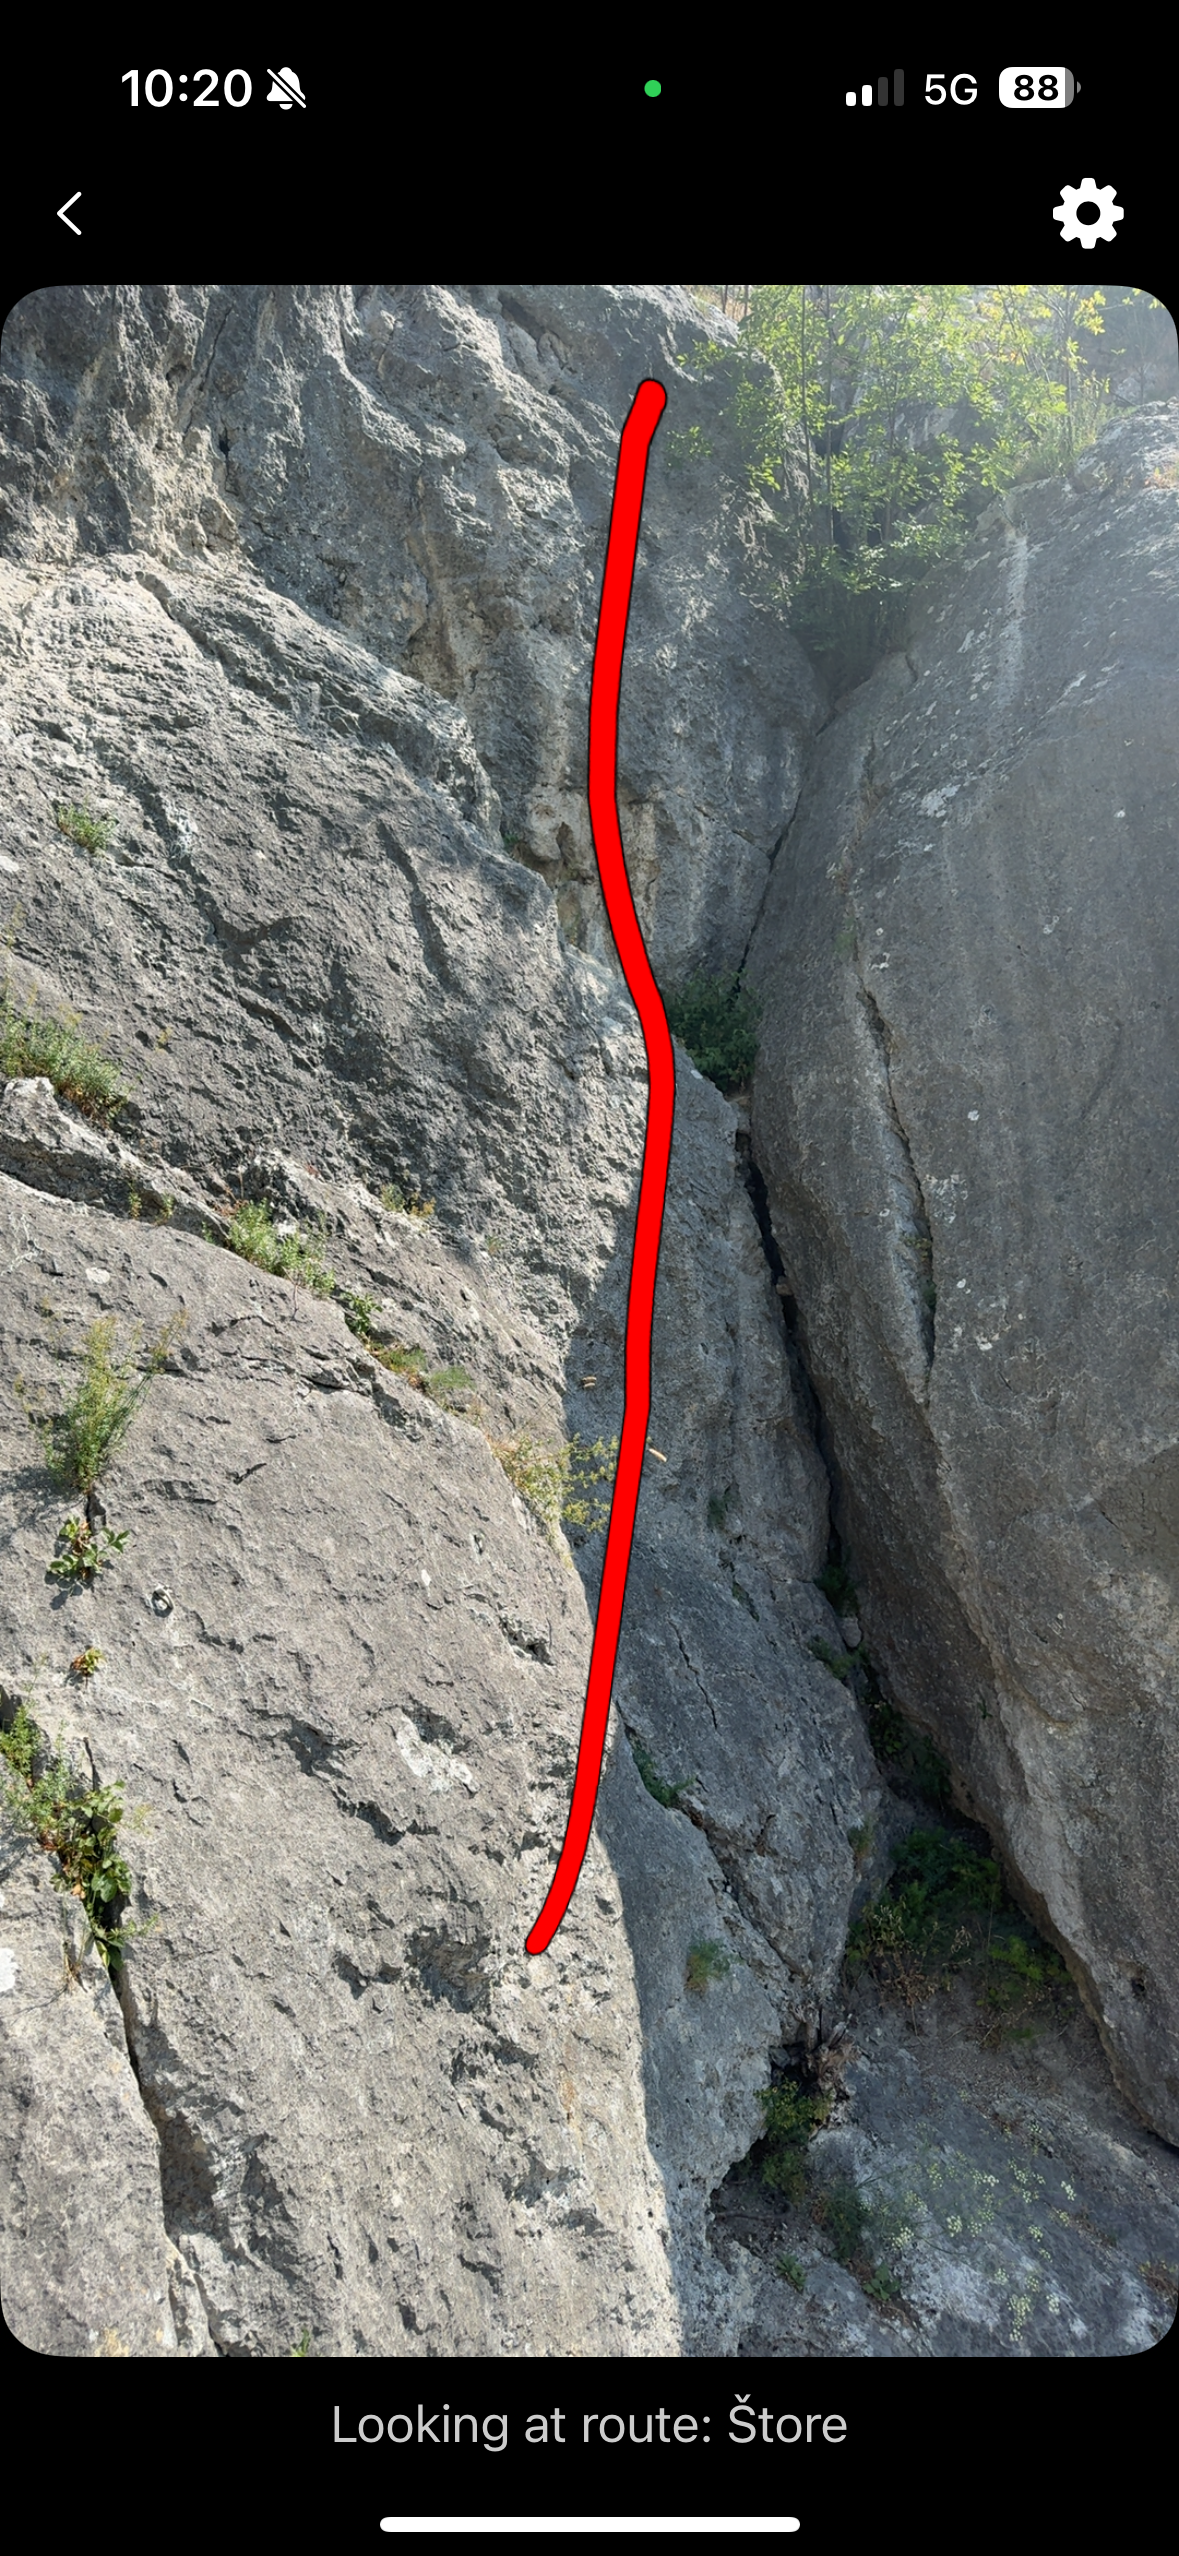
\includegraphics[width=0.3\textwidth]{images/implementacija/route_detection_auto.png}
    \caption{Automatski način rada - prepoznavanje penjačkog smjera}
    \label{fig:prepoznavanje_penjačkog_smjera_auto}
\end{figure}

Aplikacija nudi korisniku postavke za prilagodbu procesa prepozavanja. Korisnik može birati između dva glavna načina rada. U automatskom načinu rada (eng. \textit{Automatic mode}), aplikacija kontinuirano analizira slike dobivene s kamere i automatski pokušava prepoznati smjer što pruži iskustvo proširene stvarnosti (slika~\ref{fig:prepoznavanje_penjačkog_smjera_auto}). 

\begin{figure}[H]
    \centering
    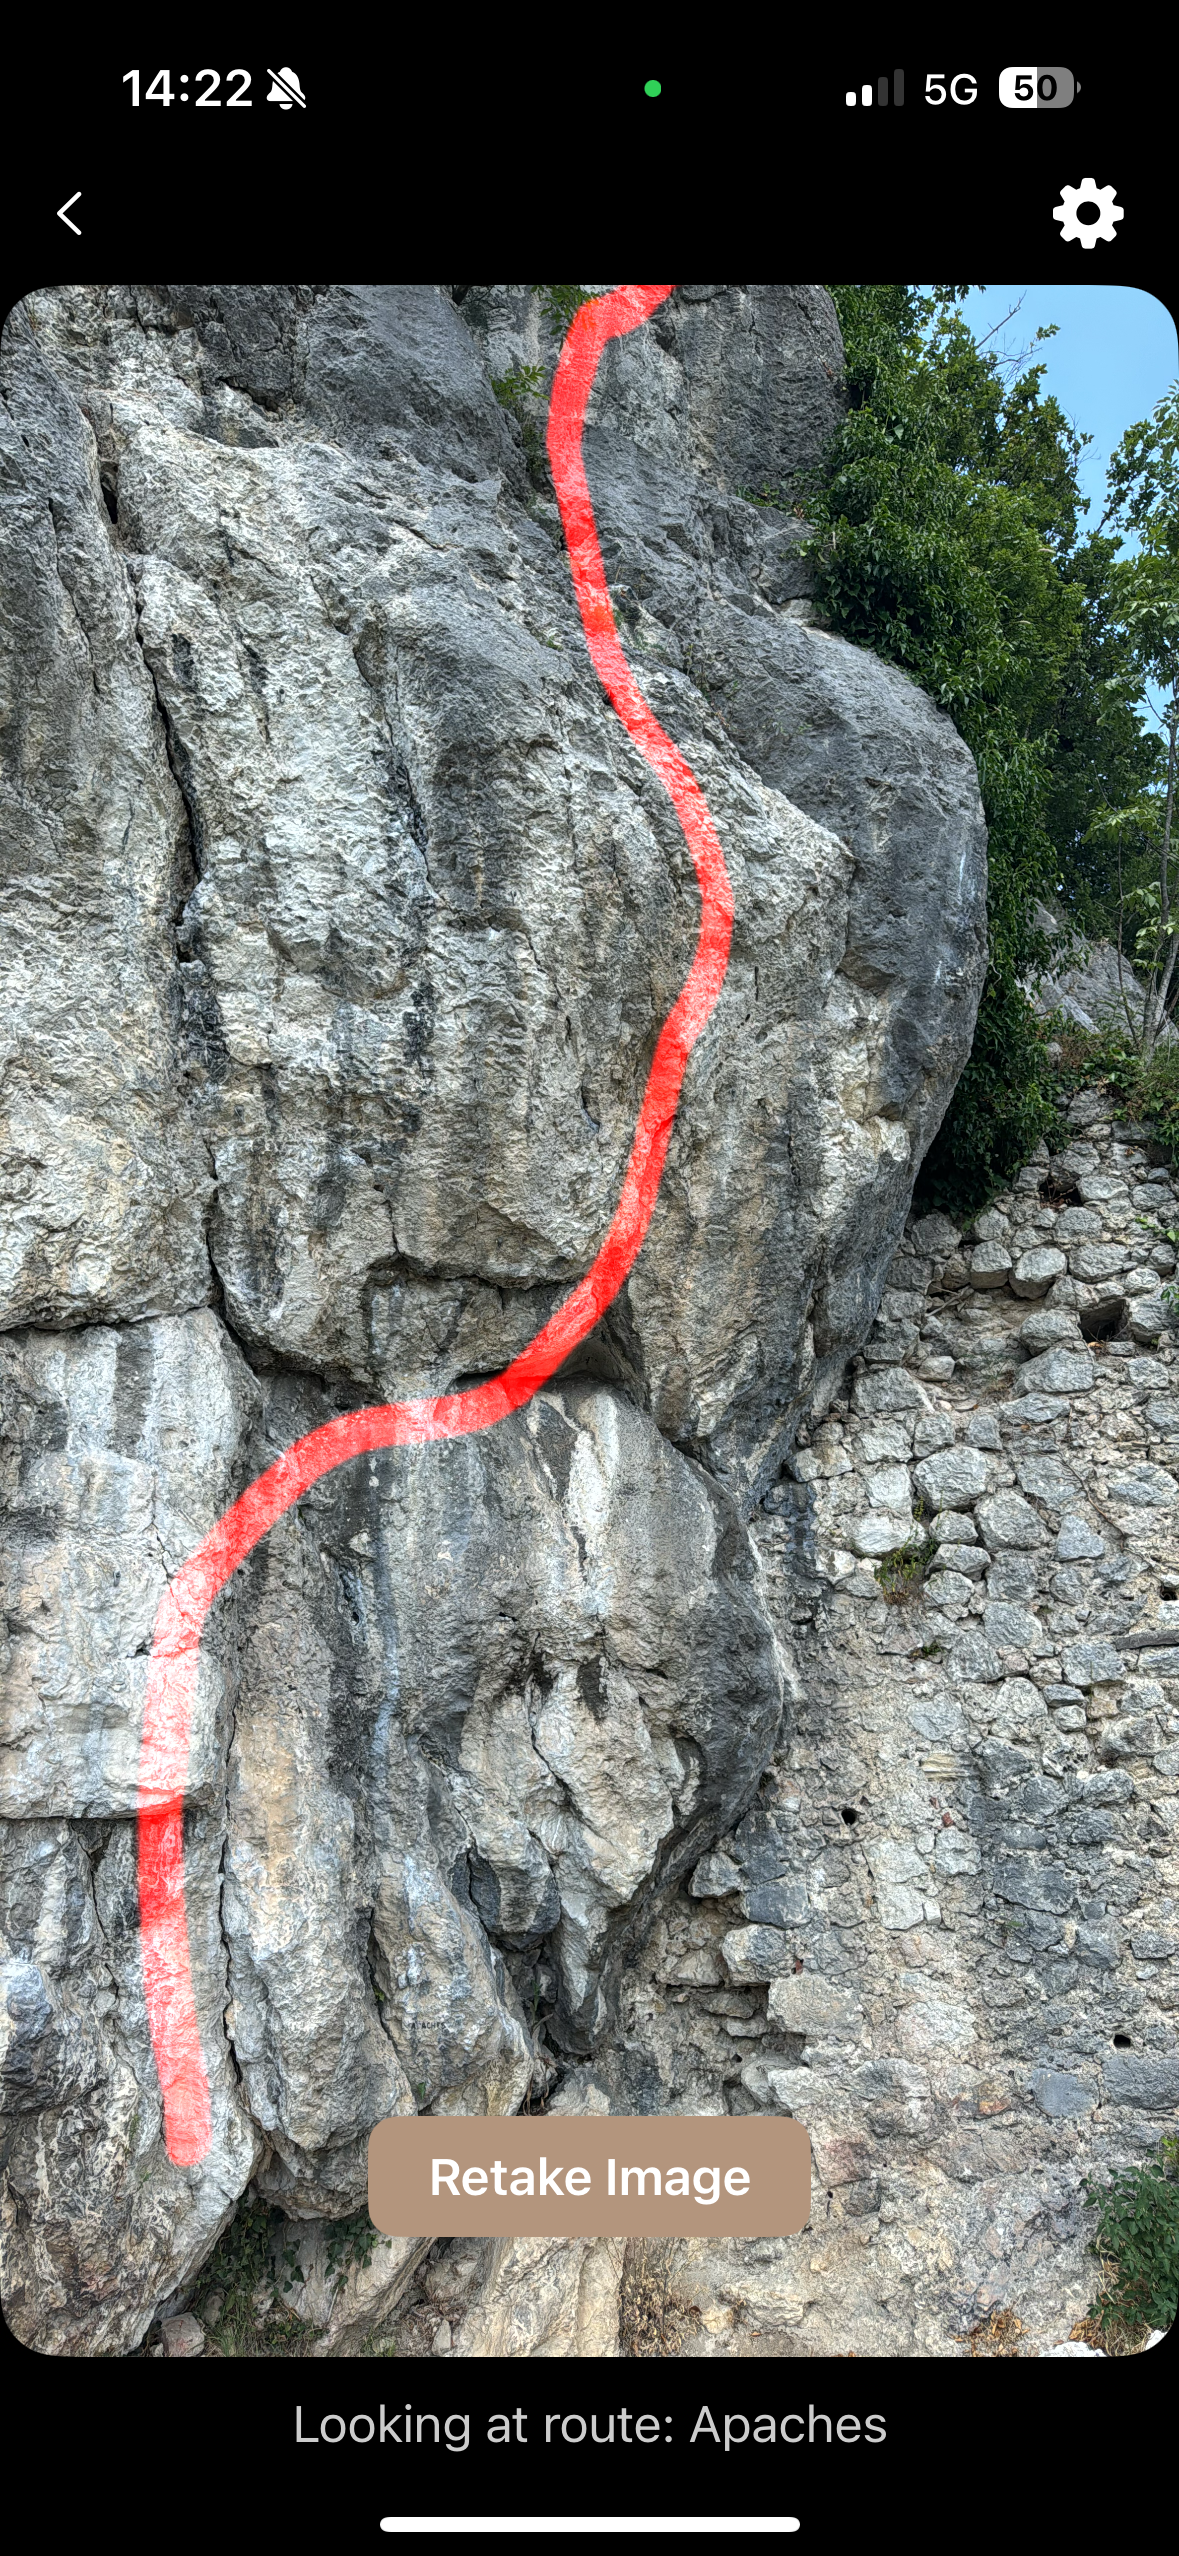
\includegraphics[width=0.3\textwidth]{images/implementacija/route_detection_manual.PNG}
    \caption{Ručni način rada - prepoznavanje penjačkog smjera}
    \label{fig:prepoznavanje_penjačkog_smjera_manual}
\end{figure}

S obzirom na računalno intezivnu prirodu tog procesa, kao alternativu kako bi se smanjila potrošnja resursa, dostupan je i ručni način rada (eng. \textit{Manual mode}). U tom načinu rada, aplikacija ne analizira slike u realnom vremenu, već korisnik samostalno snima fotografiju stijene, a proces prepoznavanja se izvršava samo na toj jednoj, statičnoj slici (slika~\ref{fig:prepoznavanje_penjačkog_smjera_manual}). 

Dodatno, korisniku su na raspolaganju dostupne i tri razine jačine prepozavanja: \textit{Low}, \textit{Medium} i \textit{High}. Ove postavke u pozadini prilagođavaju parametre algoritama kako bi se postigao kompromis između brzine i kvalitete prepoznavanja. Viša razina jačine prepoznavanja rezultira u preciznijim prepoznavanjima, ali uz veće računsko opterećenje, dok niža nudi brži rad i manju potrošnju. Ove opcije omogućuju korisniku da prilagodi proces prepozavanja prema svojim potrebama i uvjetima.